\documentclass[a4paper,12pt]{article}
\usepackage{amsmath}
\usepackage{amssymb,amsthm,graphicx}
%\usepackage{bbm} (Do not want to use these, may create conflicts)
%\usepackage{gensymb}
\usepackage{enumitem}
\usepackage{color}
\usepackage{epsfig}
\usepackage{graphics}
\usepackage{pdfpages}
\usepackage{subcaption}
\usepackage[font=small]{caption}
\usepackage[hang,flushmargin]{footmisc} 
\usepackage{float}
\usepackage{booktabs}
\usepackage[mathscr]{euscript}
\usepackage{natbib}
\usepackage{setspace}
\usepackage{mathrsfs}
\usepackage[left=2.7cm,right=2.7cm,bottom=2.7cm,top=2.7cm]{geometry}
\parindent0pt 


% General

\newcommand{\reals}{\mathbb{R}}
\newcommand{\integers}{\mathbb{Z}}
\newcommand{\naturals}{\mathbb{N}}

\newcommand{\pr}{\mathbb{P}}        % probability
\newcommand{\ex}{\mathbb{E}}        % expectation
\newcommand{\var}{\textnormal{Var}} % variance
\newcommand{\cov}{\textnormal{Cov}} % covariance

\newcommand{\law}{\mathcal{L}} % law of X
\newcommand{\normal}{N}        % normal distribution 

\newcommand{\argmax}{\textnormal{argmax}}
\newcommand{\argmin}{\textnormal{argmin}}

\newcommand{\ind}{\mathbbm{1}} % indicator function
\newcommand{\kernel}{K} % kernel function
\newcommand{\wght}{W} % kernel weight
\newcommand{\thres}{\pi} % threshold parameter


% Convergence

\newcommand{\convd}{\stackrel{d}{\longrightarrow}}              % convergence in distribution
\newcommand{\convp}{\stackrel{P}{\longrightarrow}}              % convergence in probability
\newcommand{\convas}{\stackrel{\textrm{a.s.}}{\longrightarrow}} % convergence almost surely
\newcommand{\convw}{\rightsquigarrow}                           % weak convergence


% Theorem-like declarations

\theoremstyle{plain}

\newtheorem{theorem}{Theorem}[section]
\newtheorem{prop}[theorem]{Proposition}
\newtheorem{lemma}[theorem]{Lemma}
\newtheorem{corollary}[theorem]{Corollary}
\newtheorem*{theo}{Theorem}
\newtheorem{propA}{Proposition}[section]
\newtheorem{lemmaA}[propA]{Lemma}
\newtheorem{definition}{Definition}[section]
\newtheorem{remark}{Remark}[section]
\renewcommand{\thelemmaA}{A.\arabic{lemmaA}}
\renewcommand{\thepropA}{A.\arabic{propA}}
\newtheorem*{algo}{Clustering Algorithm}


% Theorem numbering to the left

\makeatletter
\newcommand{\lefteqno}{\let\veqno\@@leqno}
\makeatother


% Heading

\newcommand{\heading}[2]
{  \setcounter{page}{1}
   \begin{center}

   \phantom{Distance to upper boundary}
   \vspace{0.5cm}

   {\LARGE \textbf{#1}}
   \vspace{0.4cm}
 
   {\LARGE \textbf{#2}}
   \end{center}
}


% Authors

\newcommand{\authors}[4]
{  \parindent0pt
   \begin{center}
      \begin{minipage}[c][2cm][c]{5cm}
      \begin{center} 
      {\large #1} 
      \vspace{0.05cm}
      
      #2 
      \end{center}
      \end{minipage}
      \begin{minipage}[c][2cm][c]{5cm}
      \begin{center} 
      {\large #3}
      \vspace{0.05cm}

      #4 
      \end{center}
      \end{minipage}
   \end{center}
}

%\newcommand{\authors}[2]
%{  \parindent0pt
%   \begin{center}
%   {\large #1} 
%   \vspace{0.1cm}
%      
%   #2 
%   \end{center}  
%}


% Version

\newcommand{\version}[1]
{  \begin{center}
   {\large #1}
   \end{center}
   \vspace{3pt}
} 










\begin{document}



\heading{Multiscale Inference for}{Nonparametric Time Trends}

\vspace{-0.5cm}

\authors{Marina Khismatullina\renewcommand{\thefootnote}{1}\footnotemark[1]}{University of Bonn}{Michael Vogt\renewcommand{\thefootnote}{2}\footnotemark[2]}{University of Bonn} 
\footnotetext[1]{Address: Bonn Graduate School of Economics, University of Bonn, 53113 Bonn, Germany. Email: \texttt{marina.k@uni-bonn.de}.}
\renewcommand{\thefootnote}{2}
\footnotetext[2]{Corresponding author. Address: Department of Economics and Hausdorff Center for Mathematics, University of Bonn, 53113 Bonn, Germany. Email: \texttt{michael.vogt@uni-bonn.de}.}
\renewcommand{\thefootnote}{\arabic{footnote}}
\setcounter{footnote}{0}

%\vspace{-0.5cm}

%\version{\today}

\vspace{-1cm}



\renewcommand{\abstractname}{}
\begin{abstract}
\noindent We develop multiscale methods to test qualitative hypotheses about nonparametric time trends. In many applications, practitioners are interested in whether the observed time series has a time trend at all, that is, whether the trend function is non-constant. Moreover, they would like to get further information about the shape of the trend function. Among other things, they would like to know in which time regions there is an upward/downward movement in the trend. When multiple time series are observed, another important question is whether the observed time series all have the same time trend. We design multiscale tests to formally approach these questions. We derive asymptotic theory for the proposed tests and investigate their finite sample performance by means of simulations. In addition, we illustrate the methods by two applications to temperature data. 
\end{abstract}

\vspace{-0.1cm}

\enlargethispage{0.25cm}
\renewcommand{\baselinestretch}{1.2}\normalsize

\textbf{Key words:} Multiscale statistics; nonparametric regression; time series errors; shape constraints; strong approximations; anti-concentration bounds.

\textbf{AMS 2010 subject classifications:} 62E20; 62G10; 62G20; 62M10. 

\vspace{-0.25cm}

\numberwithin{equation}{section}
\allowdisplaybreaks[1]




\section{Introduction}\label{sec-intro}


The analysis of time trends is an important aspect of many time series applications. In this paper, we develop new methods to analyse nonparametric time trends. 
%Alternative 1: Many time series exhibit a trending behaviour. In applications, it is often important to get a better understanding of this trending behaviour. In this paper, we develop various new methods / a toolbox of new methods to analyse nonparametric time trends. 
%Alternative 2: A wide range of time series exhibit a trending behaviour. In many applications, a particular interest lies in better understanding the trending behaviour of the observed time series. In this paper, we develop various new methods / a toolbox of new methods to analyse nonparametric time trends. 
We consider two different model settings, depending on whether a single or multiple time series are observed. When the observations come from a single time series $\{ Y_t: 1 \le t \le T \}$, we consider the model
\begin{equation}\label{model1-intro}
Y_t = m \Big( \frac{t}{T} \Big) + \varepsilon_t
\end{equation}
for $1 \le t \le T$, where $m: [0,1] \rightarrow \mathbb{R}$ is an unknown nonparametric trend function and the error terms $\varepsilon_t$ form a time series process with $\ex[\varepsilon_t] = 0$ for all $t$. When several time series $\mathcal{Y}_i = \{ Y_{it}: 1 \le t \le T \}$ are observed for $1 \le i \le n$, we similarly model each time series $\mathcal{Y}_i$ by the equation
\begin{equation}\label{model2-intro}
Y_{it} = m_i \Big( \frac{t}{T} \Big) + \alpha_i + \varepsilon_{it}
\end{equation}
for $1 \le t \le T$, where $m_i$ is a nonparametric time trend, $\alpha_i$ is a (random or deterministic) intercept and $\varepsilon_{it}$ are time series errors with $\ex[\varepsilon_{it}] = 0$ for all $t$. As usual in nonparametric regression, we let the trend functions in \eqref{model1-intro} and \eqref{model2-intro} depend on rescaled time $t/T$ rather than on real time $t$. A detailed description of models \eqref{model1-intro} and \eqref{model2-intro} is provided in Section \ref{sec-model}.

\begin{center}
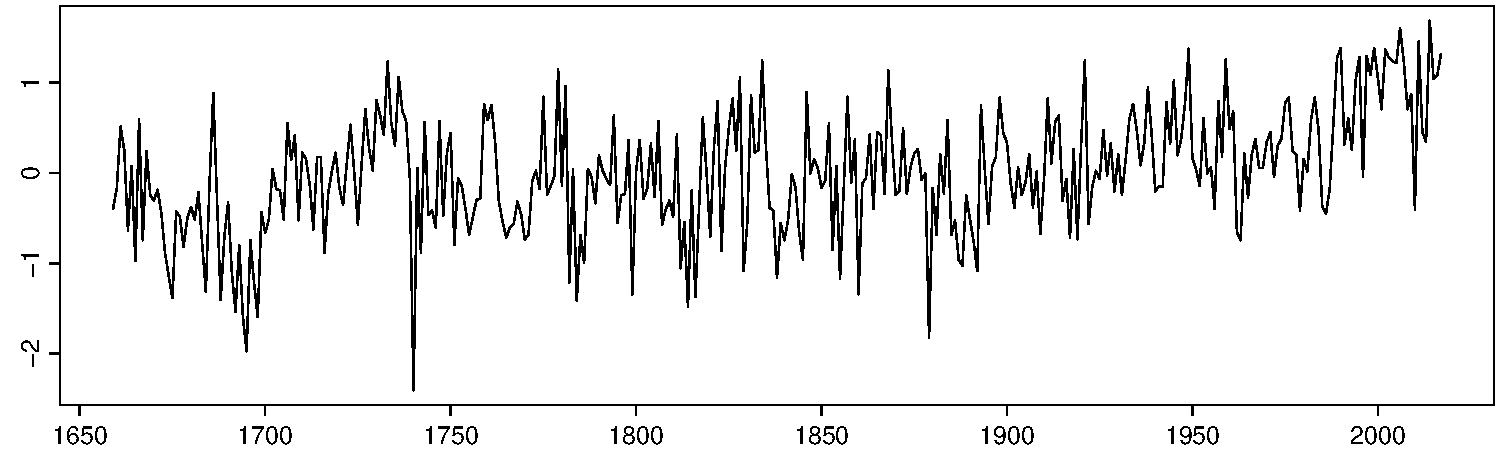
\includegraphics[width=\textwidth, clip=true]{Coding/Output/temperature_data.pdf}
\captionof{figure}{Yearly deviation from the mean temperature for England,$ \degree$ C}\label{yearly_data}%\caption{Yearly temperature data for England\label{yearly_data}}
\end{center}


Let us first have a closer look at the situation where a single time series is observed. In this case, practitioners are interested in questions such as the following: Does the observed time series have a trend at all? If so, which are the time regions where there is a strong trend? Is the trend decreasing or increasing in these regions? As an example, consider the time series plotted in Figure \ref{yearly_data} which shows the yearly mean temperature in Central England from 1659 to 2017. Climatologists are very much interested in analysing the trending behaviour of temperature time series like this; see e.g.\ \cite{Benner1999} and \cite{Rahmstorf2017}. Among other things, they would like to know whether there is an upward trend in the Central England mean temperature towards the end of the sample as visual inspection might suggest. In Section \ref{sec-test-shape}, we develop a statistical procedure to approach questions like this. Specifically, we construct a method to test the null hypothesis that there is no time trend in the data. Importantly, the proposed method does not only allow to test whether the null hypothesis of no trend is violated. It also allows to identify, with a pre-specified statistical confidence, time regions where there is an upward or downward trend in the data. As regards the temperature time series in Figure \ref{yearly_data}, we can for example claim, with a statistical confidence of approximately 95\%, that there is some upward movement of the trend in the time period between ?? and ??. This is one of the results obtained from a detailed analysis of the time series as conducted in Section \ref{sec-data}. 


Let us now turn to the situation where multiple time series of the form \eqref{model2-intro} are observed. An important question in many applications is whether the time trends $m_i$ of the various time series are all the same. When some of the time trends are different, there may still be groups of time series with the same time trend. In this case, it is often of interest to estimate the unknown groups from the data. In addition, when two time trends $m_i$ and $m_j$ are not the same, it may also be relevant to know in which time regions they differ from each other. In Section \ref{sec-test-equality}, we construct statistical methods to approach these questions. In particular, we develop a test of the hypothesis that all time trends in model \eqref{model2-intro} are the same, that is, $m_1 = m_2 = \ldots = m_n$. Similar as above, our method does not only allow to test whether the null hypothesis is violated. It also allows to detect, with a given statistical confidence, which time trends are different and in which time regions they differ from each other. Based on our test method, we further construct a clustering algorithm which estimates groups of time series with the same time trend.


%\newpage
We develop our methods and the underlying theory step by step in Sections \ref{sec-method}--\ref{sec-test-equality}. In Section \ref{sec-method}, we introduce our methods in the context of a simple baseline case. We in particular discuss the problem of testing the simple hypothesis $H_0: m = 0$ in model \eqref{model1-intro}. In Sections \ref{sec-test-shape} and \ref{sec-test-equality}, we adapt the methods and theory to the test problems we are actually interested in. To construct our methods, we build on ideas from statistical multiscale testing as developed in \cite{ChaudhuriMarron1999,ChaudhuriMarron2000}, \cite{HallHeckman2000} and \cite{DuembgenSpokoiny2001} among others. Considering the hypothesis $H_0: m = 0$ in model \eqref{model1-intro}, our test procedure can be outlined roughly as follows: In a first step, we set up statistics $\widehat{\psi}_T(u,h)$ to test the hypothesis $H_0(u,h)$ that $m = 0$ on the interval $[u-h,u+h]$. In a second step, we aggregate these statistics $\widehat{\psi}_T(u,h)$ for a wide range of different intervals $[u-h,u+h]$. We thus construct a multiscale statistic which allows to test the hypothesis $H_0(u,h)$ simultaneously for many intervals $[u-h,u+h]$. A simple approach to aggregate the statistics $\widehat{\psi}_T(u,h)$ is to take their supremum $\sup_{(u,h) \in \mathcal{G_T}} \widehat{\psi}_T(u,h)$, where $\mathcal{G}_T$ denotes the set of points $(u,h)$ which are taken into account. As shown in the seminal work of \cite{DuembgenSpokoiny2001}, this approach is suboptimal in some sense. Following their lead, we define our multiscale statistic by $\widehat{\Psi}_T = \sup_{(u,h) \in \mathcal{G_T}} \{ \widehat{\psi}_T(u,h) - \lambda(h)\}$, where $\lambda(h)$ are additive correction terms. The idea behind this additively corrected supremum statistic is discussed in detail in Section \ref{sec-method}. 


In recent years, multiscale approaches have been developed for a variety of test problems. The general idea of all these approaches is to simultaneously consider a family of test statistics for a wide range of locations $u$ and scales or bandwidths $h$. This idea has been put to work in different ways, thus resulting in different multiscale test approaches. In the regression context, \cite{ChaudhuriMarron1999,ChaudhuriMarron2000} have developed the so-called SiZer method which has been extended in various directions.
% see for example \cite{KimMarron2006} and \cite{Huckemann2016} among others. 
\cite{HallHeckman2000} have constructed a multiscale test on monotonicity of a regression function. As already discussed above, \cite{DuembgenSpokoiny2001} have developed a multiscale approach which works with additively corrected supremum statistics. They derive theoretical results in the context of  a continuous Gaussian white noise model. Their theory can be extended in a fairly straightforward way to a nonparametric regression model $Y_t = m(t/T) + \varepsilon_t$ with i.i.d.\ Subgaussian errors $\varepsilon_t$. However, it is far from trivial to extend their theory to our setting, that is, to a nonparametric regression model $Y_t = m(t/T) + \varepsilon_t$ with a general weakly dependent error process $\{\varepsilon_t\}$. To derive our theoretical results, we come up with a proof strategy which is quite different from that of \cite{DuembgenSpokoiny2001}. This strategy is of interest in itself and may be applied to other multiscale test problems. It combines strong approximation results for dependent processes as developed in \cite{BerkesLiuWu2014} with anti-concentration bounds for Gaussian vectors as derived in \cite{Chernozhukov2015}. The details are described in Section \ref{sec-method}.


Our multiscale tests complement already existing tools for analysing nonparametric time trends. The test method developed in Section \ref{sec-test-shape} provides an alternative to dependent SiZer methods as introduced in \cite{Rondonotti2004} and \cite{Rondonotti2007}. Whereas the focus of these papers is mainly methodological, we back up our multiscale test by a complete asymptotic theory which characterizes its size and power properties. The multiscale test from Section \ref{sec-test-equality} is a valuable alternative to other procedures for testing equality of time trends. To the best of our knowledge, a multiscale test for the hypothesis $H_0: m_1 = m_2 = \ldots = m_n$ in model \eqref{model2-intro} has not been developed so far in the literature. However, there are other approaches to test for equality of time trends. \cite{Vogelsang2005} and \cite{Lyubchich2016}, for example, construct tests for comparing parametric time trends, whereas \cite{DegrasWu2012} develop an $L^2$-type test for comparing nonparametric trends. One of the advantages of our multiscale approach is that it is very informative: It does not only allow to test whether the null hypothesis is violated or not. It also gives information on where violations occur, in particular, which time trends are different and in which time regions they differ. It thus provides valuable additional information for practitioners. 


We complement the theoretical analysis of the paper by a simulation study and two application examples in Sections \ref{sec-sim} and \ref{sec-data}. The simulation study investigates the finite sample properties of the test methods and the clustering algorithm from Sections \ref{sec-test-shape} and \ref{sec-test-equality}. In the first application example, we examine the temperature time series from Figure \ref{yearly_data} with the help of the methods developed in Section \ref{sec-test-shape}. In the second, we analyse temperature time series measured at 34 different weather stations located in Great Britain. We in particular apply our procedure from Section \ref{sec-test-equality} to test whether the different time series have the same trend. 



\section{The model}\label{sec-model}


We now describe the model setting in detail which was briefly outlined in the Introduction. We observe a time series $\{Y_{t,T}: 1 \le t \le T \}$ of length $T$ which satisfies the nonparametric regression equation 
\begin{equation}\label{model}
Y_{t,T} = m \Big( \frac{t}{T} \Big) + \varepsilon_t 
\end{equation}
for $1 \le t \le T$. Here, $m$ is an unknown nonparametric function defined on $[0,1]$ and $\{ \varepsilon_t: 1 \le t \le T \}$ is a zero-mean stationary error process. For simplicity, we restrict attention to equidistant design points $x_t = t/T$. However, our methods and theory can also be carried over to non-equidistant designs. The stationary error process $\{\varepsilon_t\}$ is assumed to have the following properties: 
\begin{enumerate}[label=(C\arabic*),leftmargin=1.05cm]

\item \label{C-err1} The variables $\varepsilon_t$ allow for the representation $\varepsilon_t = G(\ldots,\eta_{t-1},\eta_t,\eta_{t+1},\ldots)$, where $\eta_t$ are i.i.d.\ random variables and $G$ is a measurable function. 

\item \label{C-err2} It holds that $\| \varepsilon_t \|_q < \infty$ for some $q > 4$, where $\| \varepsilon_t \|_q = (\ex|\varepsilon_t|^q)^{1/q}$. 

\end{enumerate}
Following \cite{Wu2005}, we impose conditions on the dependence structure of the error process $\{\varepsilon_t\}$ in terms of the physical dependence measure $d_{t,q} = \| \varepsilon_t - \varepsilon_t^\prime \|_q$, where $\varepsilon_t^\prime = G(\ldots,\eta_{-1},\eta_0^\prime,\eta_1,\ldots,\eta_{t-1},\eta_t,\eta_{t+1},\ldots)$ with $\{\eta_t^\prime\}$ being an i.i.d.\ copy of $\{\eta_t\}$. In particular, we assume the following: 
\begin{enumerate}[label=(C\arabic*),leftmargin=1.05cm]
\setcounter{enumi}{2}

\item \label{C-err3} Define $\Theta_{t,q} = \sum\nolimits_{|s| \ge t} d_{s,q}$ for $t \ge 0$. It holds that 
\[ \Theta_{t,q} = O \big( t^{-\tau_q} (\log t)^{-A} \big), \] 
where $A > \frac{2}{3} (1/q + 1 + \tau_q)$ and $\tau_q = \{q^2 - 4 + (q-2) \sqrt{q^2 + 20q + 4}\} / 8q$. 

\end{enumerate}
The conditions \ref{C-err1}--\ref{C-err3} are fulfilled by a wide range of stationary processes $\{\varepsilon_t\}$. As a first example, consider linear processes of the form $\varepsilon_t = \sum\nolimits_{i=0}^{\infty} c_i \eta_{t-i}$ with $\| \varepsilon_t \|_q < \infty$, where $c_i$ are absolutely summable coefficients and $\eta_t$ are i.i.d.\ innovations with $\ex[\eta_t] = 0$ and $\| \eta_t\|_q < \infty$. Trivially, \ref{C-err1} and \ref{C-err2} are fulfilled in this case. Moreover, if $|c_i| = O(\rho^i)$ for some $\rho \in (0,1)$, then \ref{C-err3} is easily seen to be satisfied as well. As a special case, consider an ARMA process $\{\varepsilon_t\}$ of the form $\varepsilon_t + \sum\nolimits_{i=1}^p a_i \varepsilon_{t-i} = \eta_t + \sum\nolimits_{j=1}^r b_j \eta_{t-j}$  with $\| \varepsilon_t \|_q < \infty$, where $a_1,\ldots,a_p$ and $b_1,\ldots,b_r$ are real-valued parameters. As before, we let $\eta_t$ be i.i.d.\ innovations with $\ex[\eta_t] = 0$ and $\| \eta_t\|_q < \infty$. Moreover, as usual, we suppose that the complex polynomials $A(z) = 1 + \sum\nolimits_{j=1}^p a_jz^j$ and $B(z) = 1 + \sum\nolimits_{j=1}^r b_jz^j$ do not have any roots in common. If $A(z)$ does not have any roots inside the unit disc, then the ARMA process $\{ \varepsilon_t \}$ is stationary and causal. Specifically, it has the representation $\varepsilon_t = \sum\nolimits_{i=0}^{\infty} c_i \eta_{t-i}$ with $|c_i| = O(\rho^i)$ for some $\rho \in (0,1)$, implying that \ref{C-err1}--\ref{C-err3} are fulfilled. The results in \cite{WuShao2004} show that condition \ref{C-err3} (as well as the other two conditions) is not only fulfilled for linear time series processes but also for a variety of non-linear processes. 



\section{The multiscale test}\label{sec-method}


In this section, we introduce our multiscale method to test for local increases/decreases of the trend function $m$ and analyse its theoretical properties. We assume throughout that $m$ is continuously differentiable on $[0,1]$. The test problem under consideration can be formulated as follows: Let $H_0(u,h)$ be the hypothesis that $m$ is constant on the interval $[u-h,u+h]$. Since $m$ is differentiable, $H_0(u,h)$ can be reformulated as
\[ H_0(u,h): m^\prime(w) = 0 \text { for all } w \in [u-h,u+h], \]
where $m^\prime$ is the first derivative of $m$. We want to test the hypothesis $H_0(u,h)$ not only for a single interval $[u-h,u+h]$ but simultaneously for many different intervals. The overall null hypothesis is thus given by
\[ H_0: \text{ The hypothesis } H_0(u,h) \text{ holds true for all } (u,h) \in \mathcal{G}_T, \]
where $\mathcal{G}_T$ is some large set of points $(u,h)$. The details on the set $\mathcal{G}_T$ are discussed at the end of Section \ref{subsec-method-stat} below. Note that $\mathcal{G}_T$ in general depends on the sample size $T$, implying that the null hypothesis $H_0 = H_{0,T}$ depends on $T$ as well. We thus consider a sequence of null hypotheses $\{H_{0,T}: T = 1,2,\ldots \}$ as $T$ increases. For simplicity of notation, we however suppress the dependence of $H_0$ on $T$. In Sections \ref{subsec-method-stat} and \ref{subsec-method-test}, we step by step construct the multiscale test of the hypothesis $H_0$. The theoretical properties of the test are analysed in Section \ref{subsec-method-theo}. 


\subsection{Construction of the multiscale statistic}\label{subsec-method-stat}


We first construct a test statistic for the hypothesis $H_0(u,h)$, where $[u-h,u+h]$ is a given interval. To do so, we consider the kernel average
\begin{equation*}
\widehat{\psi}_T(u,h) = \sum\limits_{t=1}^T w_{t,T}(u,h) Y_{t,T}, 
\end{equation*}
where $w_{t,T}(u,h)$ is a kernel weight and $h$ is the bandwidth. In order to avoid boundary issues, we work with a local linear weighting scheme. We in particular set 
\begin{equation}\label{weights}
w_{t,T}(u,h) = \frac{\Lambda_{t,T}(u,h)}{ \{\sum\nolimits_{t=1}^T \Lambda_{t,T}(u,h)^2 \}^{1/2} }, 
\end{equation}
where
\[ \Lambda_{t,T}(u,h) = K\Big(\frac{\frac{t}{T}-u}{h}\Big) \Big[ S_{T,0}(u,h) \Big(\frac{\frac{t}{T}-u}{h}\Big) - S_{T,1}(u,h) \Big], \]
$S_{T,\ell}(u,h) = (Th)^{-1} \sum\nolimits_{t=1}^T K(\frac{\frac{t}{T}-u}{h}) (\frac{\frac{t}{T}-u}{h})^\ell$ for $\ell = 0,1,2$ and $K$ is a kernel function with the following properties: 
\begin{enumerate}[label=(C\arabic*),leftmargin=1.05cm]
\setcounter{enumi}{3}
\item \label{C-ker} The kernel $K$ is non-negative, symmetric about zero and integrates to one. Moreover, it has compact support $[-1,1]$ and is Lipschitz continuous, that is, $|K(v) - K(w)| \le C |v-w|$ for any $v,w \in \reals$ and some constant $C > 0$. 
\end{enumerate} 
The kernel average $\widehat{\psi}_T(u,h)$ is nothing else than a rescaled local linear estimator of the derivative $m^\prime(u)$ with bandwidth $h$.\footnote{Alternatively to the local linear weights defined in \eqref{weights}, we could also work with the weights $w_{t,T}(u,h) = K^\prime( h^{-1} [u - t/T] )/ \{ \sum\nolimits_{t=1}^T  K^\prime( h^{-1}[u - t/T] )^2 \}^{1/2}$, where the kernel function $K$ is assumed to be differentiable and $K^\prime$ is its derivative. We however prefer to use local linear weights as these have superior theoretical properties at the boundary.}  


A test statistic for the hypothesis $H_0(u,h)$ is given by the normalized kernel average $\widehat{\psi}_T(u,h)/\widehat{\sigma}$, where $\widehat{\sigma}^2$ is an estimator of the long-run variance $\sigma^2 = \sum\nolimits_{\ell=-\infty}^{\infty} \cov(\varepsilon_0,\varepsilon_\ell)$ of the error process $\{\varepsilon_t\}$. The problem of estimating $\sigma^2$ is discussed in detail in Section \ref{sec-error-var}. For the time being, we suppose that $\widehat{\sigma}^2$ is an estimator with reasonable theoretical properties. Specifically, we assume that $\widehat{\sigma}^2 = \sigma^2 + o_p(\rho_T)$ with $\rho_T = o(1/\log T)$. This is a fairly weak condition which is in particular satisfied by the estimators of $\sigma^2$ analysed in Section \ref{sec-error-var}. The kernel weights $w_{t,T}(u,h)$ are chosen such that in the case of independent errors $\varepsilon_t$, $\var(\widehat{\psi}_T(u,h)) = \sigma^2$ for any location $u$ and bandwidth $h$, where the long-run error variance $\sigma^2$ simplifies to $\sigma^2 = \var(\varepsilon_t)$. In the more general case that the error terms satisfy the weak dependence conditions from Section \ref{sec-model}, it holds that $\var(\widehat{\psi}_T(u,h)) = \sigma^2 + o(1)$ for any location $u$ and any bandwidth $h$ with $h \rightarrow 0$ and $Th \rightarrow \infty$. Hence, for sufficiently large sample sizes $T$, the test statistic $\widehat{\psi}_T(u,h)/\widehat{\sigma}$ has approximately unit variance for any such $u$ and $h$.


We now combine the test statistics $\widehat{\psi}_T(u,h)/\widehat{\sigma}$ for a wide range of different locations $u$ and bandwidths or scales $h$. There are different ways to do so, leading to different types of multiscale statistics. Our multiscale statistic is defined as
\begin{equation}\label{multiscale-stat}
\widehat{\Psi}_T = \max_{(u,h) \in \mathcal{G}_T} \Big\{ \Big|\frac{\widehat{\psi}_T(u,h)}{\widehat{\sigma}}\Big| - \lambda(h) \Big\}, 
\end{equation} 
where $\lambda(h) = \sqrt{2 \log \{ 1/(2h) \}}$ and $\mathcal{G}_T$ is the set of points $(u,h)$ that are taken into consideration. The details on the set $\mathcal{G}_T$ are given below. As can be seen, the statistic $\widehat{\Psi}_T$ does not simply aggregate the individual statistics $\widehat{\psi}_T(u,h)/\widehat{\sigma}$ by taking the supremum over all points $(u,h) \in \mathcal{G}_T$ as in more traditional multiscale approaches. We rather calibrate the statistics $\widehat{\psi}_T(u,h)/\widehat{\sigma}$ that correspond to the bandwidth $h$ by subtracting the additive correction term $\lambda(h)$. This approach was pioneered by \cite{DuembgenSpokoiny2001} and has been used in numerous other studies since then; see e.g.\ \cite{Duembgen2002}, \cite{Rohde2008}, \cite{DuembgenWalther2008}, \cite{RufibachWalther2010}, \cite{SchmidtHieber2013} and \cite{EckleBissantzDette2017}. 
%aggregation scheme has been introduced by ?? and has been used in a variety of other multiscale approaches since then; cp.\ e.g.\ the multiscale tests in ??. 
%We rather follow the approach pioneered by \cite{DuembgenSpokoiny2001} and subtract the additive correction term $\lambda(h)$ from the statistics $\widehat{\psi}_T(u,h)/\widehat{\sigma}$ that correspond to the bandwidth level $h$. 
To see the heuristic idea behind the additive correction $\lambda(h)$, consider for a moment the uncorrected statistic
\[ \widehat{\Psi}_{T,\text{uncorrected}} = \max_{(u,h) \in \mathcal{G}_T} \Big|\frac{\widehat{\psi}_T(u,h)}{\widehat{\sigma}}\Big| \]
and suppose that the hypothesis $H_0(u,h)$ is true for all $(u,h) \in \mathcal{G}_T$. For simplicity, assume that the errors $\varepsilon_t$ are i.i.d.\ normally distributed and neglect the estimation error in $\widehat{\sigma}$, that is, set $\widehat{\sigma} = \sigma$. Moreover, suppose that the set $\mathcal{G}_T$ only consists of the points $(u_k,h_\ell) = ((2k - 1)h_\ell,h_\ell)$ with $k = 1,\ldots,\lfloor 1/2h_\ell \rfloor$ and $\ell = 1,\ldots,L$. In this case, we can write
\[ \widehat{\Psi}_{T,\text{uncorrected}} = \max_{1 \le \ell \le L} \max_{1 \le k \le \lfloor 1/2h_\ell \rfloor} \Big|\frac{\widehat{\psi}_T(u_k,h_\ell)}{\sigma}\Big|. \]
Under our simplifying assumptions, the statistics $\widehat{\psi}_T(u_k,h_\ell)/\sigma$ with $k = 1,\ldots,\lfloor 1/2h_\ell \rfloor$ are independent and standard normal for any given bandwidth $h_\ell$. Since the maximum over $\lfloor 1/2h \rfloor$ independent standard normal random variables is $\lambda(h) + o_p(1)$ as $h \rightarrow 0$, we obtain that $\max_{k} \widehat{\psi}_T(u_k,h_\ell)/\sigma$ is approximately of size $\lambda(h_\ell)$ for small bandwidths $h_\ell$. As $\lambda(h) \rightarrow \infty$ for $h \rightarrow 0$, this implies that $\max_{k} \widehat{\psi}_T(u_k,h_\ell)/\sigma$ tends to be much larger in size for small than for large bandwidths $h_\ell$. As a result, the stochastic behaviour of the uncorrected statistic $\widehat{\Psi}_{T,\text{uncorrected}}$ tends to be dominated by the statistics $\widehat{\psi}_T(u_k,h_\ell)$ corresponding to small bandwidths $h_\ell$. The additively corrected statistic $\widehat{\Psi}_T$, in contrast, puts the statistics $\widehat{\psi}_T(u_k,h_\ell)$ corresponding to different bandwidths $h_\ell$ on a more equal footing, thus counteracting the dominance of small bandwidth values. 


The multiscale statistic $\widehat{\Psi}_T$ simultaneously takes into account all locations $u$ and bandwidths $h$ with $(u,h) \in \mathcal{G}_T$. Throughout the paper, we suppose that $\mathcal{G}_T$ is some subset of $\mathcal{G}_T^{\text{full}} = \{ (u,h): u = t/T \text{ for some } 1 \le t \le T \text{ and } h \in [h_{\min},h_{\max}] \}$, where $h_{\min}$ and $h_{\max}$ denote some minimal and maximal bandwidth value, respectively. For our theory to work, we require the following conditions to hold:
\begin{enumerate}[label=(C\arabic*),leftmargin=1.05cm]
\setcounter{enumi}{4}

\item \label{C-grid} $|\mathcal{G}_T| = O(T^\theta)$ for some arbitrarily large but fixed constant $\theta > 0$, where $|\mathcal{G}_T|$ denotes the cardinality of $\mathcal{G}_T$. 

\item \label{C-h} $h_{\min} \gg T^{-(1-\frac{2}{q})} \log T$, that is, $h_{\min} / \{ T^{-(1-\frac{2}{q})} \log T \} \rightarrow \infty$ with $q > 4$ defined in \ref{C-err2} and $h_{\max} \le 1/2$.

\end{enumerate}
According to \ref{C-grid}, the number of points $(u,h)$ in $\mathcal{G}_T$ should not grow faster than $T^\theta$ for some arbitrarily large but fixed $\theta > 0$. This is a fairly weak restriction as it allows the set $\mathcal{G}_T$ to be extremely large as compared to the sample size $T$. For example, we may work with the set 
\begin{align*}
\mathcal{G}_T = \big\{ & (u,h): u = t/T \text{ for some } 1 \le t \le T \text{ and } h \in [h_{\min},h_{\max}] \\ & \text{ with } h = t/T \text{ for some } 1 \le t \le T  \big\},
\end{align*}
which contains more than enough points $(u,h)$ for most practical applications. Condition \ref{C-h} imposes some restrictions on the minimal and maximal bandwidths $h_{\min}$ and $h_{\max}$. These conditions are fairly weak, allowing us to choose the bandwidth window $[h_{\min},h_{\max}]$ extremely large. The lower bound on $h_{\min}$ depends on the parameter $q$ defined in \ref{C-err2} which specifies the number of existing moments for the error terms $\varepsilon_t$. As one can see, we can choose $h_{\min}$ to be of the order $T^{-1/2}$ for any $q > 4$. Hence, we can let $h_{\min}$ converge to $0$ very quickly even if only the first few moments of the error terms $\varepsilon_t$ exist. If all moments exist (i.e.\ $q = \infty$), we even get that $h_{\min}$ may converge to $0$ almost as quickly as $T^{-1} \log T$. Moreover, the maximal bandwidth $h_{\max}$ is not even required to converge to $0$, which implies that we can pick it very large.


\begin{remark}
The above construction of the multiscale statistic can be easily adapted to hypotheses other than $H_0$. To do so, one simply needs to replace the kernel weights $w_{t,T}(u,h)$ defined in \eqref{weights} by appropriate versions which are suited to test the hypothesis of interest. For example, if one wants to test for local convexity/concavity of $m$, one may define the kernel weights $w_{t,T}(u,h)$ such that the kernel average $\widehat{\psi}_T(u,h)$ is a (rescaled) estimator of the second derivative of $m$ at the location $u$ with bandwidth $h$. 
\end{remark}


\subsection{The test procedure}\label{subsec-method-test}


In order to formulate a test for the null hypothesis $H_0$, we still need to specify a critical value. To do so, we define the statistic
\begin{equation}\label{Phi-statistic}
\Phi_T = \max_{(u,h) \in \mathcal{G}_T} \Big\{ \Big|\frac{\phi_T(u,h)}{\sigma}\Big| - \lambda(h) \Big\},
\end{equation} 
where $\phi_T(u,h) = \sum\nolimits_{t=1}^T w_{t,T}(u,h) \, \sigma Z_t$ and $Z_t$ are independent standard normal random variables. The statistic $\Phi_T$ can be regarded as a Gaussian version of the test statistic $\widehat{\Psi}_T$ under the null hypothesis $H_0$. Let $q_T(\alpha)$ be the $(1-\alpha)$-quantile of $\Phi_T$. Importantly, the quantile $q_T(\alpha)$ can be computed by Monte Carlo simulations and can thus be regarded as known. Our multiscale test of the hypothesis $H_0$ is now defined as follows: For a given significance level $\alpha \in (0,1)$, we reject $H_0$ if $\widehat{\Psi}_T > q_T(\alpha)$. 


\subsection{Theoretical properties of the test}\label{subsec-method-theo}


In order to examine the theoretical properties of our multiscale test, we introduce the auxiliary multiscale statistic 
\begin{align}
\widehat{\Phi}_T 
% & = \max_{(u,h) \in \mathcal{G}_T} \Big\{ \Big| \frac{\widehat{\psi}_T(u,h) - \ex \widehat{\psi}_T(u,h)}{\widehat{\sigma}} \Big| - \lambda(h) \Big\} \nonumber \\
 & = \max_{(u,h) \in \mathcal{G}_T} \Big\{ \Big| \frac{\widehat{\phi}_T(u,h)}{\widehat{\sigma}} \Big| - \lambda(h) \Big\} \label{Phi-hat-statistic}
\end{align}
with $\widehat{\phi}_T(u,h) = \widehat{\psi}_T(u,h) - \ex [\widehat{\psi}_T(u,h)] = \sum\nolimits_{t=1}^T w_{t,T}(u,h) \varepsilon_t$. The following result is central to the theoretical analysis of our multiscale test. According to it, the (known) quantile $q_T(\alpha)$ of the Gaussian statistic $\Phi_T$ defined in Section \ref{subsec-method-test} can be used as a proxy for the $(1-\alpha)$-quantile of the multiscale statistic $\widehat{\Phi}_T$.
\begin{theorem}\label{theo-stat}
Let \ref{C-err1}--\ref{C-h} be fulfilled and assume that $\widehat{\sigma}^2 = \sigma^2 + o_p(\rho_T)$ with $\rho_T = o(1/\log T)$. Then 
\[ \pr \big( \widehat{\Phi}_T \le q_T(\alpha) \big) = (1 - \alpha) + o(1). \]
\end{theorem}
A full proof of Theorem \ref{theo-stat} is given in the Appendix. 
%We here shortly outline the proof strategy which may be applied to other multiscale test problems for dependent data. The strategy splits up into two main steps. 
%We here shortly outline the proof strategy, which is of broader interest as it can potentially be applied in the context of a variety of other statistical multiscale problems. The strategy splits up into two main steps: 
We here shortly outline the proof strategy, which splits up into two main steps. 
In the first, we replace the statistic $\widehat{\Phi}_T$ for each $T \ge 1$ by a statistic $\widetilde{\Phi}_T$ with the same distribution as $\widehat{\Phi}_T$ and the property that 
\begin{equation}\label{eq-theo-stat-strategy-step1}
\big| \widetilde{\Phi}_T - \Phi_T \big| = o_p(\delta_T),
\end{equation}
where $\delta_T = o(1)$ and the Gaussian statistic $\Phi_T$ is defined in Section \ref{subsec-method-test}. We thus replace the statistic $\widehat{\Phi}_T$ by an identically distributed version which is close to a Gaussian statistic whose distribution is known. To do so, we make use of strong approximation theory for dependent processes as derived in \cite{BerkesLiuWu2014}. In the second step, we show that 
\begin{equation}\label{eq-theo-stat-strategy-claim}
\sup_{x \in \reals} \big| \pr(\widetilde{\Phi}_T \le x) - \pr(\Phi_T \le x) \big| = o(1), 
\end{equation}
which immediately implies the statement of Theorem \ref{theo-stat}. Importantly, the convergence result \eqref{eq-theo-stat-strategy-step1} is not sufficient for establishing \eqref{eq-theo-stat-strategy-claim}. Put differently, the fact that $\widetilde{\Phi}_T$ can be approximated by $\Phi_T$ in the sense that $\widetilde{\Phi}_T - \Phi_T = o_p(\delta_T)$ does not imply that the distribution of $\widetilde{\Phi}_T$ is close to that of $\Phi_T$ in the sense of \eqref{eq-theo-stat-strategy-claim}. For \eqref{eq-theo-stat-strategy-claim} to hold, we additionally require the distribution of $\Phi_T$ to have some sort of continuity property. Specifically, we prove that 
\begin{equation}\label{eq-theo-stat-strategy-step2}
\sup_{x \in \reals} \pr \big( |\Phi_T - x| \le \delta_T \big) = o(1),
\end{equation}
which says that $\Phi_T$ does not concentrate too strongly in small regions of the form $[x-\delta_T,x+\delta_T]$. The main tool for verifying \eqref{eq-theo-stat-strategy-step2} are anti-concentration results for Gaussian random vectors as derived in \cite{Chernozhukov2015}. The claim \eqref{eq-theo-stat-strategy-claim} can be proven by using \eqref{eq-theo-stat-strategy-step1} together with \eqref{eq-theo-stat-strategy-step2}, which in turn yields Theorem \ref{theo-stat}. 


The main idea of our proof strategy is to combine strong approximation theory with anti-concentration bounds for Gaussian random vectors to show that the quantiles of the multiscale statistic $\widehat{\Phi}_T$ can be proxied by those of a Gaussian analogue. This strategy is quite general in nature and may be applied to other multiscale problems for dependent data. Strong approximation theory has also been used to investigate multiscale tests for independent data; see e.g.\ 
%the multiscale analysis of densities in a deconvolution model in 
\cite{SchmidtHieber2013}. However, it has not been combined with anti-concentration results to approximate the quantiles of the multiscale statistic. As an alternative to strong approximation theory, \cite{EckleBissantzDette2017} and \cite{ProkschWernerMunk2018} have recently used Gaussian approximation results derived in \cite{Chernozhukov2014, Chernozhukov2017} to analyse multiscale tests for independent data. Even though it might be possible to adapt these techniques to the case of dependent data, this is not trivial at all as part of the technical arguments and the Gaussian approximation tools strongly rely on the assumption of independence. 


We now investigate the theoretical properties of our multiscale test with the help of Theorem \ref{theo-stat}. The first result is an immediate consequence of Theorem \ref{theo-stat}. It says that the test has the correct (asymptotic) size. 
\begin{prop}\label{prop-test-1}
Let the conditions of Theorem \ref{theo-stat} be satisfied. Under the null hypothesis $H_0$, it holds that 
\[ \pr \big( \widehat{\Psi}_T \le q_T(\alpha) \big) = (1 - \alpha) + o(1). \]
\end{prop}
The second result characterizes the power of the multiscale test against local alternatives. To formulate it, we consider any sequence of functions $m = m_T$ with the following property: There exists $(u,h) \in \mathcal{G}_T$ with $[u-h,u+h] \subseteq [0,1]$ such that 
\begin{equation}\label{loc-alt}
m_T^\prime(w) \ge c_T \sqrt{\frac{\log T}{Th^3}} \quad \text{for all } w \in [u-h,u+h], 
\end{equation}
where $\{c_T\}$ is any sequence of positive numbers with $c_T \rightarrow \infty$. Alternatively to \eqref{loc-alt}, we may also assume that $-m_T^\prime(w) \ge c_T \sqrt{\log T/(Th^3)}$ for all $w \in [u-h,u+h]$. According to the following result, our test has asymptotic power $1$ against local alternatives of the form \eqref{loc-alt}. 
\begin{prop}\label{prop-test-2}
Let the conditions of Theorem \ref{theo-stat} be satisfied and consider any sequence of functions $m_T$ with the property \eqref{loc-alt}. Then 
\[ \pr \big( \widehat{\Psi}_T \le q_T(\alpha) \big) = o(1). \]
\end{prop}
The proof of Proposition \ref{prop-test-2} can be found in the Appendix. To formulate the next result, we define 
\begin{align*}
\Pi_T^\pm   & = \big\{ I_{u,h} = [u-h,u+h]: (u,h) \in \mathcal{A}_T^\pm \big\} \\
\Pi_T^+ & = \big\{ I_{u,h} = [u-h,u+h]: (u,h) \in \mathcal{A}_T^+ \text{ and } I_{u,h} \subseteq [0,1] \big\} \\
\Pi_T^- & = \big\{ I_{u,h} = [u-h,u+h]: (u,h) \in \mathcal{A}_T^- \text{ and } I_{u,h} \subseteq [0,1] \big\} 
\end{align*}
together with 
\begin{align*}
\mathcal{A}_T^\pm & = \Big\{ (u,h) \in \mathcal{G}_T: \Big|\frac{\widehat{\psi}_T(u,h)}{\widehat{\sigma}}\Big| > q_T(\alpha) + \lambda(h) \Big\} \\ 
\mathcal{A}_T^+  & = \Big\{ (u,h) \in \mathcal{G}_T: \frac{\widehat{\psi}_T(u,h)}{\widehat{\sigma}} > q_T(\alpha) + \lambda(h) \Big\} \\ 
\mathcal{A}_T^-  & = \Big\{ (u,h) \in \mathcal{G}_T: -\frac{\widehat{\psi}_T(u,h)}{\widehat{\sigma}} > q_T(\alpha) + \lambda(h) \Big\}. 
\end{align*}
$\Pi_T^\pm$ is the collection of intervals $I_{u,h} = [u-h,u+h]$ for which the (corrected) test statistic $|\widehat{\psi}_T(u,h)/\widehat{\sigma}| - \lambda(h)$ lies above the critical value $q_T(\alpha)$. $\Pi_T^+$ and $\Pi_T^-$ can be interpreted analogously but take into account the sign of the statistic $\widehat{\psi}_T(u,h)/\widehat{\sigma}$. With this notation at hand, we consider the events 
\begin{align*}
E_T^\pm & = \Big\{ \forall I_{u,h} \in \Pi_T^\pm: m^\prime(v) \ne 0 \text{ for some } v \in I_{u,h} = [u-h,u+h] \Big\} \\
E_T^+  & = \Big\{ \forall I_{u,h} \in \Pi_T^+: m^\prime(v) > 0 \text{ for some } v \in I_{u,h} = [u-h,u+h] \Big\} \\
E_T^-  & = \Big\{ \forall I_{u,h} \in \Pi_T^-: m^\prime(v) < 0 \text{ for some } v \in I_{u,h} = [u-h,u+h] \Big\}.
\end{align*}
$E_T^\pm$ ($E_T^+$, $E_T^-$) is the event that the function $m$ is non-constant (increasing, decreasing) on all intervals $I_{u,h} \in \Pi_T^\pm$ ($\Pi_T^+$, $\Pi_T^-$). More precisely, $E_T^\pm$ ($E_T^+$, $E_T^-$) is the event that for each interval $I_{u,h} \in \Pi_T^\pm$ ($\Pi_T^+$, $\Pi_T^-$), there is a subset $J_{u,h} \subseteq I_{u,h}$ with $m$ being a non-constant (increasing, decreasing) function on $J_{u,h}$. We can make the following formal statement about the events $E_T^\pm$, $E_T^+$ and $E_T^-$ whose proof is given in the Appendix. 
\begin{prop}\label{prop-test-3}
Let the conditions of Theorem \ref{theo-stat} be fulfilled. Then for $\ell \in \{ \pm,+,-\}$, it holds that
\[ \pr \big( E_T^\ell \big) \ge (1-\alpha) + o(1). \]
\end{prop}
According to Proposition \ref{prop-test-3}, we can make uniform confidence statements of the following form: With (asymptotic) probability $\ge (1-\alpha)$, the trend function $m$ is non-constant (increasing, decreasing) on some part of the interval $I_{u,h}$ for all $I_{u,h} \in \Pi_T$ ($\Pi_T^+$, $\Pi_T^-$). Hence, our multiscale procedure allows to identify, with a pre-specified confidence, time regions where there is an increase/decrease in the time trend $m$. 


\begin{remark}
Unlike $\Pi_T$, the sets $\Pi_T^+$ and $\Pi_T^-$ only contain intervals $I_{u,h} = [u-h,u+h]$ which are subsets of $[0,1]$. We thus exclude points $(u,h) \in \mathcal{A}_T^+$ and $(u,h) \in \mathcal{A}_T^-$ which lie at the boundary, that is, for which $I_{u,h} \nsubseteq [0,1]$. The reason is as follows: Let $(u,h) \in \mathcal{A}_T^+$ with $I_{u,h} \nsubseteq [0,1]$. Our technical arguments allow us to say, with asymptotic confidence $\ge 1 - \alpha$, that $m^\prime(v) \ne 0$ for some $v \in I_{u,h}$. However, we cannot say whether $m^\prime(v) > 0$ or $m^\prime(v) < 0$, that is, we cannot make confidence statements about the sign. Crudely speaking, the problem is that the local linear weights $w_{t,T}(u,h)$ behave quite differently at boundary points $(u,h)$ with $I_{u,h} \nsubseteq [0,1]$. As a consequence, we can include boundary points $(u,h)$ in $\Pi_T$ but not in $\Pi_T^+$ and $\Pi_T^-$.
\end{remark}
 

The statement of Proposition \ref{prop-test-3} suggests to graphically present the results of our multiscale test by plotting the intervals $I_{u,h} \in \Pi_T^\ell$ for $\ell \in \{\pm, +,-\}$, that is, by plotting the intervals where (with asymptotic confidence $\ge 1-\alpha$) our test detects a violation of the null hypothesis. The drawback of this graphical presentation is that the number of intervals in $\Pi_T^\ell$ is often quite large. To obtain a better graphical summary of the results, we replace $\Pi_T^\ell$ by a subset $\Pi_T^{\ell,\min}$ which is constructed as follows: As in \cite{Duembgen2002}, we call an interval $I_{u,h} \in \Pi_T^\ell$ minimal if there is no other interval $I_{u^\prime,h^\prime} \in \Pi_T^\ell$ with $I_{u^\prime,h^\prime} \subset I_{u,h}$. Let $\Pi_T^{\ell,\min}$ be the set of all minimal intervals in $\Pi_T^\ell$ for $\ell \in \{\pm, +,-\}$ and define the events
\begin{align*}
E_T^{\pm,\min} & = \Big\{ \forall I_{u,h} \in \Pi_T^{\pm,\min}: m^\prime(v) \ne 0 \text{ for some } v \in I_{u,h} = [u-h,u+h] \Big\} \\
E_T^{+,\min} & = \Big\{ \forall I_{u,h} \in \Pi_T^{+,\min}: m^\prime(v) > 0 \text{ for some } v \in I_{u,h} = [u-h,u+h] \Big\} \\ 
E_T^{-,\min} & = \Big\{ \forall I_{u,h} \in \Pi_T^{-,\min}: m^\prime(v) < 0 \text{ for some } v \in I_{u,h} = [u-h,u+h] \Big\}.  
\end{align*}
It is easily seen that $E_T^\ell = E_T^{\ell,\min}$ for $\ell \in \{\pm, +,-\}$. Hence, by Proposition \ref{prop-test-3}, it holds that 
\[ \pr \big(E_T^{\ell,\min}\big) \ge (1-\alpha) + o(1) \] 
for $\ell \in \{\pm, +,-\}$. This suggests to plot the minimal intervals in $\Pi_T^{\ell,\min}$ rather than the whole collection of intervals $\Pi_T^\ell$ as a graphical summary of the test results. We in particular use this way of presenting the test results in our applications of Section \ref{sec-data}. 



\section{Estimation of the long-run error variance}\label{sec-error-var}


We now discuss how to estimate the long-run error variance $\sigma^2 = \sum\nolimits_{\ell=-\infty}^{\infty} \cov(\varepsilon_0,\varepsilon_{\ell})$ in model \eqref{model}. There are two broad classes of estimators: residual- and difference-based estimators. Residual-based methods proceed by applying standard methods for estimating $\sigma^2$ to the time series of residuals $\widehat{\varepsilon}_t = Y_{t,T} - \widehat{m}_h(t/T)$, where $\widehat{m}_h$ is a nonparametric estimator of $m$ with the bandwidth or smoothing parameter $h$. Difference-based methods attempt to estimate $\sigma^2$ by applying statistical methods to certain differences of the observed time series $\{Y_{t,T}\}$, for example, to the first differences $\Delta Y_{t,T} = Y_{t,T} - Y_{t-1,T}$. Notably, difference-based methods do not involve a nonparametric estimator of $m$ and thus do not require to specify a smoothing parameter $h$ for the estimation of $m$. 


\subsection{General weakly dependent error terms}


We first consider a general stationary error process $\{ \varepsilon_t \}$. In particular, we do not impose any time series model such as a moving average (MA) or an autoregressive (AR) model on $\{\varepsilon_t\}$ but only require that $\{\varepsilon_t\}$ satisfies certain weak dependence conditions such as those from Section \ref{sec-model}. 


A residual-based estimator of $\sigma^2$ can be obtained as follows: Estimating $\sigma^2$ amounts to estimating the spectral density $f_\varepsilon$ of the error process $\{\varepsilon_t\}$ at frequency $0$ (assuming that $f_\varepsilon$ exists). We may thus apply existing methods for estimating $f_\varepsilon(0)$ such as developed in \cite{LiuWu2010} to the time series of residuals $\widehat{\varepsilon}_t = Y_{t,T} - \widehat{m}_h(t/T)$. Note that the resulting estimator of $\sigma^2$ will depend on two different smoothing parameters: one for the preliminary estimation of $m$ and one for the estimation of the nonparametric density $f_\varepsilon$ at the point $0$. 
Alternatively, $\sigma^2$ may be estimated by difference-based methods. We briefly describe an approach which goes back to ideas from \cite{Hart1989, Hart1991}. Consider the differences $\Delta Y_{t,T} = Y_{t,T} - Y_{t-1,T}$ and let $I_\Delta$ be (a tapered version of) the periodogram of $\{\Delta_t\}$.\footnote{\cite{Hart1989, Hart1991} actually considered the differences $\Delta_2 Y_{t,T} = Y_{t+1,T} - 2Y_{t,T} + Y_{t-1,T}$. However, the idea behind the estimation method is the same no matter whether $\Delta Y_{t,T}$ or $\Delta_2 Y_{t,T}$ is used.} Following \cite{Hart1989, Hart1991}, the autocovariances $\gamma_\varepsilon(\ell) = \cov(\varepsilon_0,\varepsilon_\ell)$ can be estimated by 
\[ \widehat{\gamma}_\varepsilon(\ell) = \frac{4\pi}{T} \sum\limits_{j = j(\delta)}^{\lceil T/2 \rceil} \cos (\omega_j \ell) |1 - \exp(-i \omega_j)|^{-2} I_\Delta(\omega_j), \]
where $\omega_j = 2\pi j/T$, $j(\delta) = \lceil n\delta/(2\pi) \rceil$ and $\delta$ is a tuning parameter satisfying $\delta \rightarrow 0$ and $T \delta \rightarrow \infty$. We may now employ HAC-type estimation procedures, as discussed in \cite{Andrews1991} or \cite{DeJong2000}, to estimate $\sigma^2$ by 
\[ \widehat{\sigma}^2 = \sum_{|\ell| \le b_T} W \Big( \frac{\ell}{b_T} \Big) \, \widehat{\gamma}_\varepsilon(\ell), \]
where $W: [-1,1] \rightarrow \reals$ is a kernel of Bartlett or flat-top type and $b_T$ is a bandwidth parameter with $b_T \rightarrow \infty$ and $b_T/T \rightarrow 0$. 


Estimating the long-run error variance of $\{ \varepsilon_t \}$ under general conditions is a notoriously difficult problem and estimators of $\sigma^2$ such as those described above tend to be quite imprecise. Moreover, no matter whether residual- or difference-based methods are used, the estimators depend on one or several smoothing parameters which are quite difficult to select. For these reasons, we follow authors such as \cite{Hart1991, Hart1994} and \cite{Hall2003} and impose a time series model on the error terms $\{\varepsilon_t\}$ in model \eqref{model}. Estimating $\sigma^2$ under the restrictions of such a model may of course create some misspecification bias. However, as long as the model gives a reasonable approximation to the true error process, the produced estimates of $\sigma^2$ can be expected to be fairly reliable even though they are a bit biased. 


\subsection{Autoregressive error terms}\label{subsec-error-var-ar}


A number of studies have analysed the problem of estimating $\sigma^2$ in model \eqref{model} with MA($q$) or, more generally, $q$-dependent error terms. Difference-based estimators of $\sigma^2$ for this case have been proposed in \cite{MuellerStadtmueller1988}, \cite{Herrmann1992} and \cite{Munk2017} among others. Under the assumption of $q$-dependence, $\gamma_\varepsilon(\ell) := \cov(\varepsilon_0,\varepsilon_{\ell}) = 0$ for all $|\ell| > q$. Even though $q$-dependent time series are a reasonable error model in some applications, the condition that $\gamma_\varepsilon(\ell)$ is exactly equal to $0$ for sufficiently large lags $\ell$ is quite restrictive in many situations. Presumably the most widely used error model in practice is an AR($p$) process. Methods to estimate $\sigma^2$ in model \eqref{model} with AR($p$) errors have for example been proposed in \cite{Hall2003} and \cite{ShaoYang2011}. 


In what follows, we introduce a simple estimator of $\sigma^2$ for the AR($p$) case which is completely free of tuning parameters. As we will see, the estimation method extends to ARMA($p,q$) errors in a straightforward way. As in \cite{Hall2003}, we consider the following situation: $\{\varepsilon_t\}$ is a stationary and causal AR($p$) process of the form 
\begin{equation}\label{AR-errors} 
\varepsilon_t = \sum_{j=1}^p a_j \varepsilon_{t-j} + \eta_t, 
\end{equation} 
where $a_1,\ldots,a_p$ are unknown parameters and $\eta_t$ are i.i.d.\ innovations with $\ex[\eta_t] = 0$ and $\ex[\eta_t^2] = \sigma_\eta^2$. The AR order $p$ is known and $m$ is Lipschitz continuous on $[0,1]$, that is, $|m(u) - m(v)| \le L|u-v|$ for all $u,v \in [0,1]$ and some constant $L < \infty$. 


Our estimation method relies on the following simple observation: If $\{\varepsilon_t\}$ is an AR($p$) process of the form \eqref{AR-errors}, then the time series $\{ \Delta \varepsilon_t \}$ of the differences $\Delta \varepsilon_t = \varepsilon_t - \varepsilon_{t-1}$ is an ARMA($p,1$) process of the form 
\begin{equation}\label{AR-diff-errors} 
\Delta \varepsilon_t - \sum_{j=1}^p a_j \Delta \varepsilon_{t-j} = \eta_t - \eta_{t-1}. 
\end{equation}
For completeness, we give a formal proof of \eqref{AR-diff-errors} in the Appendix. The differences $\Delta \varepsilon_t$ of the unobserved error process are close to the differences $\Delta Y_{t,T} = Y_{t,T} - Y_{t-1,T}$ of the observed time series in the sense that 
\begin{equation}\label{diff-Y-eps}
\Delta Y_{t,T} = \big[\varepsilon_t  - \varepsilon_{t-1} \big] + \Big[ m \Big(\frac{t}{T}\Big) - m \Big(\frac{t-1}{T}\Big) \Big] = \Delta \varepsilon_t + O \Big( \frac{1}{T} \Big).  
\end{equation} 
Taken together, \eqref{AR-diff-errors} and \eqref{diff-Y-eps} imply that the differenced time series $\{ \Delta Y_{t,T} \}$ is approximately an ARMA($p,1$) process of the form \eqref{AR-diff-errors}. This suggests to estimate the parameters $a_1,\ldots,a_p$ and the residual variance $\sigma_\eta^2$ by applying standard methods for ARMA process to the time series $\{ \Delta Y_{t,T} \}$. Since $\sigma^2 = \sigma^2_\eta ( 1-\sum_{j=1}^p a_j)^{-2}$ in the AR($p$) case, this immediately yields an estimator of $\sigma^2$. 


Our estimators of $a_1,\ldots,a_p$ and $\sigma_\eta^2$ are constructed as follows: Let $\gamma(\ell) = \cov(\Delta \varepsilon_t,$ $\Delta \varepsilon_{t-\ell})$ and define $b_0 = 1$, $b_1 = -1$ as well as $c_{-1} = 0$, $c_0 = 1$ and $c_1 = a_1 + b_1$. The ARMA($p,1$) process $\{ \Delta \varepsilon_t \}$ satisfies the Yule-Walker equations
\begin{align}
\gamma(\ell) - \sum\limits_{j=1}^p a_j \gamma(\ell-j) & = \sigma_\eta^2 \sum_{k=\ell}^1 c_{k-\ell} b_k \hspace{-2cm} & & \text{for } \ell = 0,1 \label{diff-eq-1} \\
\gamma(\ell) - \sum\limits_{j=1}^p a_j \gamma(\ell-j) & = 0 \hspace{-2cm} & & \text{for } \ell \ge 2; \label{diff-eq-2}  
\end{align}
cp.\ \S3.3 in \cite{BrockwellDavis1991}. The equations \eqref{diff-eq-2} for $2 \le \ell \le p+1$ can be written more compactly as $\boldsymbol{\gamma}_p = \boldsymbol{\Gamma}_p \, \boldsymbol{a}$, where $\boldsymbol{a} = (a_1,\ldots,a_p)^\top$,
\[ \boldsymbol{\gamma}_p = 
\begin{pmatrix} 
\gamma(2) \\ \gamma(3) \\ \vdots \\ \gamma(p-1)    
\end{pmatrix}
\qquad \text{and} \qquad  
\boldsymbol{\Gamma}_p = 
\begin{pmatrix} 
\gamma(1) & \gamma(0)   & \dots   & \gamma(p-2) \\
\gamma(2) & \gamma(1)   & \dots   & \gamma(p-3) \\
\vdots    & \vdots      &  \ddots & \vdots      \\
\gamma(p) & \gamma(p-1) & \dots   & \gamma(1)
\end{pmatrix}. \] 
To obtain an estimator of $\boldsymbol{a}$, we replace the unknown quantities in the equation $\boldsymbol{a} = \boldsymbol{\Gamma}_p^{-1} \boldsymbol{\gamma}_p$ by estimators. In particular, we define $\widehat{\boldsymbol{a}} = (\widehat{a}_1,\ldots,\widehat{a}_p)^\top$ by 
\begin{equation}\label{est-AR-par}  
\widehat{\boldsymbol{a}} = \widehat{\boldsymbol{\Gamma}}_p^{-1} \widehat{\boldsymbol{\gamma}}_p,
\end{equation}
where $\widehat{\boldsymbol{\gamma}}_p$ and $\widehat{\boldsymbol{\Gamma}}_p$ are defined analogously as $\boldsymbol{\gamma}_p$ and $\boldsymbol{\Gamma}_p$ with $\gamma(\ell)$ replaced by the sample autocovariance 
\begin{equation}\label{est-autocov}
\widehat{\gamma}(\ell) = \frac{1}{T} \sum\limits_{t=1}^{T-|\ell|} \Delta Y_{t,T} \, \Delta Y_{t+|\ell|,T}. 
\end{equation}
We next use equation \eqref{diff-eq-1} with $\ell = 1$ to obtain that $\sigma_\eta^2 = \sum_{j=1}^p a_j \gamma(1-j) - \gamma(1)$. This suggests to estimate the innovation variance $\sigma_\eta^2$ by 
\begin{equation}\label{est-var-eta}
\widehat{\sigma}_\eta^2 = \sum_{j=1}^p \widehat{a}_j \widehat{\gamma}(1-j) - \widehat{\gamma}(1).
\end{equation}
Recalling that $\sigma^2 = \sigma^2_\eta ( 1-\sum_{j=1}^p a_j)^{-2}$, we finally define our estimator of the long-run error variance $\sigma^2$ by 
\begin{equation}\label{est-lrv}
\widehat{\sigma}^2 = \widehat{\sigma}^2_\eta \Big( 1-\sum_{j=1}^p \widehat{a}_j\Big)^{-2}. 
\end{equation}  
The estimators $\widehat{\boldsymbol{a}}$, $\widehat{\sigma}_\eta^2$ and $\widehat{\sigma}^2$ have the following formal properties. 
\begin{prop}\label{prop-lrv}
Let $\{ \varepsilon_t \}$ be a stationary and causal AR($p$) process of the form \eqref{AR-errors} and let $m$ be Lipschitz. Then ??. 
\end{prop}


We briefly compare our estimators to competing methods from the literature. Presumably closest to our method is the procedure of \cite{Hall2003}. Nevertheless, it differs from our approach in several respects, the most important difference being the following: In order to construct their estimators, \cite{Hall2003} need to compute the differences $\Delta_\ell \varepsilon_t = \varepsilon_t - \varepsilon_{t-\ell}$ for $L_1 \le \ell \le L_2$, where $L_1$ and $L_2$ are two tuning parameters that are required to fulfill the conditions $L_1 / \log T \rightarrow \infty$ and $L_2 = O(T^{1/2})$. Our approach, in contrast, is only based on the first differences $\Delta \varepsilon_t = \varepsilon_t - \varepsilon_{t-1}$ and does not involve any tuning parameters. The advantage of being completely free of tuning parameters comes, of course, at some cost: Our estimators of the AR parameters $a_1,\ldots,a_p$ (and thus also those of $\sigma_\eta^2$ and $\sigma^2$) are $\sqrt{T}$-consistent as are the estimators of \cite{Hall2003}. However, in general, they have a somewhat larger asymptotic variance than those of \cite{Hall2003} and in this sense are a bit less efficient. Hence, we trade a bit of efficiency for the practical advantage of not having to choose any tuning parameter. 
%(ii) In order to compute the innovation variance $\sigma_\eta^2$, the procedure of \cite{Hall2003} requires to compute the parameters $\widetilde{d}_1, \widetilde{d}_2, \ldots$ in the expansion $1 + \sum_{\ell=1}^\infty \widehat{d}_\ell z^\ell = (1 - \sum_{j=1}^p \widetilde{a}_j z^j )^{-1}$, where $\widetilde{a}_j$ denote the estimators of $a_j$ from \cite{Hall2003}. Whereas it is trivial to compute the coefficients $\widetilde{d}_1, \widetilde{d}_2, \ldots$ in the AR($1$) case, this becomes quite tedious for $p > 1$. 


Before we close the section, we discuss how to extend our methods to the ARMA case. To do so, suppose that $\{ \varepsilon_t \}$ is a stationary and causal ARMA($p,q$) process of the form 
\begin{equation}\label{ARMA-errors} 
\varepsilon_t - \sum_{j=1}^p a_j \varepsilon_{t-j} = \eta_t + \sum\limits_{k=1}^q b_k \eta_{t-k}, 
\end{equation} 
where $a_1,\ldots,a_p$ and $b_1,\ldots,b_q$ are unknown parameters and the innovations $\eta_t$ are as above. Similarly as in the AR($p$) case, we can show the following: If $\{\varepsilon_t\}$ is an ARMA($p,q$) process of the form \eqref{ARMA-errors}, then the time series $\{ \Delta \varepsilon_t \}$ of the differences $\Delta \varepsilon_t = \varepsilon_t - \varepsilon_{t-1}$ is an ARMA($p,q+1$) process of the form 
\begin{equation}\label{ARMA-diff-errors} 
\Delta \varepsilon_t - \sum_{j=1}^p a_j \Delta \varepsilon_{t-j} = \eta_t + \sum\limits_{k=1}^{q+1} d_k \eta_{t-k},
\end{equation}
where $d_k = b_k + b_{k-1}$ for $1 \le k \le q$ with $b_0 = 1$ and $d_{q+1} = b_q$. The unknown parameters $a_1,\ldots,a_p$, $d_1,\ldots,d_{q+1}$ and $\sigma_\eta^2$ can be estimated similarly as above by using the Yule-Walker equations corresponding to model \eqref{ARMA-diff-errors}. Once we have computed estimators for $d_1,\ldots,d_{q+1}$, we trivially get estimators for $b_1,\ldots,b_q$ as well and can estimate the long-run error variance $\sigma^2$ with the help of the formula $\sigma^2 = \sigma^2_\eta (1+\sum_{k=1}^q b_k)^2 / ( 1-\sum_{j=1}^p a_j)^2$. 


% Procedure of van Keilegom and Hall:

%The differencing approach presented above can be extended to more complicated error structures. For the case of $k$-dependent error terms, estimators for $\sigma^2$ have been proposed by \cite{MuellerStadtmueller1988}, \cite{Herrmann1992} and \cite{Munk2017} among others. We here focus attention on the case of autoregressive error terms. Specifically, we suppose that $\{\varepsilon_t\}$ is an AR($p$) process of the form $\varepsilon_t = \sum_{j=1}^p a_j \varepsilon_{t-j} + \eta_t$, where $a_1,\ldots,a_p$ are unknown parameters and $\eta_t$ are i.i.d.\ innovations with $\ex[\eta_t] = 0$ and $\ex[\eta_t^2] = \sigma_\eta^2$. Throughout the discussion, we assume that $\{\varepsilon_t\}$ is a stationary and causal AR($p$) process of known order $p$ with finite fourth moment $\ex[\varepsilon_t^4] < \infty$. A difference-based method to estimate the long-run variance $\sigma^2$ of the AR($p$) error process $\{\varepsilon_t\}$ in model \eqref{model} has been developed in \cite{Hall2003}. Their estimator $\widehat{\sigma}^2$ is constructed in the following three steps: 
%\vspace{10pt}

%\textit{Step 1.} We first set up an estimator of the autocovariance $\gamma(\ell) = \cov(\varepsilon_t,\varepsilon_{t+\ell})$ for a given lag $\ell$. As in the case of independent errors, it holds that $D_\ell Y_t = D_\ell \varepsilon_t + O(\ell/T)$ uniformly over $t$ provided that $m$ is Lipschitz. This together with the fact that $\ex[ \{  D_\ell \varepsilon_t \}^2 ] / 2 = \gamma(0) - \gamma(\ell)$ motivates to estimate $\gamma(0)$ by
%$\widehat{\gamma}(0) = \frac{1}{L_2-L_1+1}\sum_{r=L_1}^{L_2}\frac{1}{2(T-r)}\sum_{t=r+1}^T\{D_rY_t\}^2$, 
%where $L_1\le L_2$ are tuning parameters which are discussed in more detail below. Moreover, an estimator of $\gamma(\ell)$ for $1 \le \ell \le p$ is given by 
%$\widehat{\gamma}(\ell) = \widehat{\gamma}(0) - \frac{1}{2(T-\ell)}\sum_{t=\ell+1}^T \{D_\ell Y_t\}^2$.
%As $\gamma(\ell) = \gamma(-\ell)$, we finally set $\widehat{\gamma}(-\ell) = \widehat{\gamma}(\ell)$ for $1 \le \ell \le p$. 
%\vspace{10pt}

%\textit{Step 2.} We next estimate the AR coefficients $(a_1,\ldots,a_p)^\top$ by the Yule-Walker estimators $(\widehat{a}_1,\ldots,\widehat{a}_p)^\top = \widehat{\Gamma}^{-1} (\widehat{\gamma}(1), \ldots, \widehat{\gamma}(p))^\top$, where $\widehat{\Gamma} = \{ \widehat{\gamma}(|k-\ell|) \}_{1 \le k,\ell \le p}$. 
%\vspace{10pt}

%\textit{Step 3.} Let $\widehat{d}_0 = 1$ and define the parameters $\widehat{d}_1, \widehat{d}_2, \ldots$ by the equation $1 + \sum_{\ell=1}^\infty \widehat{d}_\ell z^\ell = (1 - \sum_{j=1}^p \widehat{a}_j z^j )^{-1}$. In the AR($1$) case $\varepsilon_t = a \varepsilon_{t-1} + \eta_t$ with $|a| < 1$, for instance, it holds that $\sum_{\ell = 0}^\infty \widehat{a}^\ell z^\ell = (1 - \widehat{a}z)^{-1}$ and thus $\widehat{d}_\ell = \widehat{a}^\ell$ for $\ell \ge 1$. The variance $\sigma_\eta^2 = \ex[\eta_t^2]$ of the innovations can be estimated by $\widehat{\sigma}_\eta^2 = \widehat{\gamma}(0) / (\sum_{\ell=0}^\infty \widehat{d}_\ell^2)$. With this notation at hand, we define 
%\[\widehat{\sigma}^2 = \widehat{\sigma}^2_\eta \Big( 1-\sum_{j=1}^p \widehat{a}_j\Big)^{-2} \]
%to be our estimator of the long-run error variance $\sigma^2$.
%\vspace{10pt}

%The estimator $\widehat{\sigma}^2$ depends on the two tuning parameters $L_1$ and $L_2$ which are required to compute $\widehat{\gamma}(0)$. To better understand the role of these tuning parameters, let us have a closer look at the estimator $\widehat{\gamma}(0)$. As $\ex[ \{ D_\ell Y_t \}^2 ]/2 = \ex[ \{ D_\ell \varepsilon_t \}^2 ]/2 + O( \{\ell/T\}^2 ) = \gamma(0) - \gamma(\ell) + O( \{\ell/T\}^2 )$, it can be easily shown that
%\[ \ex\big[\widehat{\gamma}(0)\big] = \gamma(0) - \frac{1}{L_2-L_1+1}\sum_{r=L_1}^{L_2} \gamma(r) + O\Big( \Big\{\frac{L_2}{T} \Big\}^2 \Big). \]
%The two bias terms $\sum_{r=L_1}^{L_2} \gamma(r) / (L_2-L_1+1)$ and $O(\{ L_2/T \}^2)$ can be asymptotically neglected if we choose the tuning parameters $L_1$ and $L_2$ appropriately. Since $\{ \varepsilon_t\}$ is an AR($p$) process, the autocovariances $\gamma(r)$ decay exponentially fast to zero as $r \rightarrow \infty$. Hence, the bias term $\sum_{r=L_1}^{L_2} \gamma(r) / (L_2-L_1+1)$ is asymptotically negligible if $L_1$ grows sufficiently fast with the sample size $T$. Due to the exponential decay of the autocovariances, it in particular suffices to assume that $L_1/\log T \rightarrow \infty$. For the second bias term  $O(\{ L_2/T \}^2)$ to be asymptotically negligible, we need to assume that $L_2$ grows more slowly than the sample size $T$. In practice, $L_1$ should be chosen so large that the autocovariances $\gamma(\ell)$ with $\ell \ge L_1$ can be expected to be close to zero, ensuring that the bias term $\sum_{r=L_1}^{L_2} \gamma(r) / (L_2-L_1+1)$ is sufficiently small. The choice of $L_2$ can be expected to be less important in practice than that of $L_1$ as long as we do not pick $L_2$ too close to the sample size $T$. As pointed out in \cite{Hall2003}, it can be shown that $\widehat{\sigma}^2 = \sigma^2 + O_p(T^{-1/2})$ provided that $L_1/\log T \rightarrow \infty$ and $L_2 = O(T^{1/2})$. 



\subsection{Analysis of UK weather station data}\label{subsec-data-2} 

\begin{figure}[t]
\centering
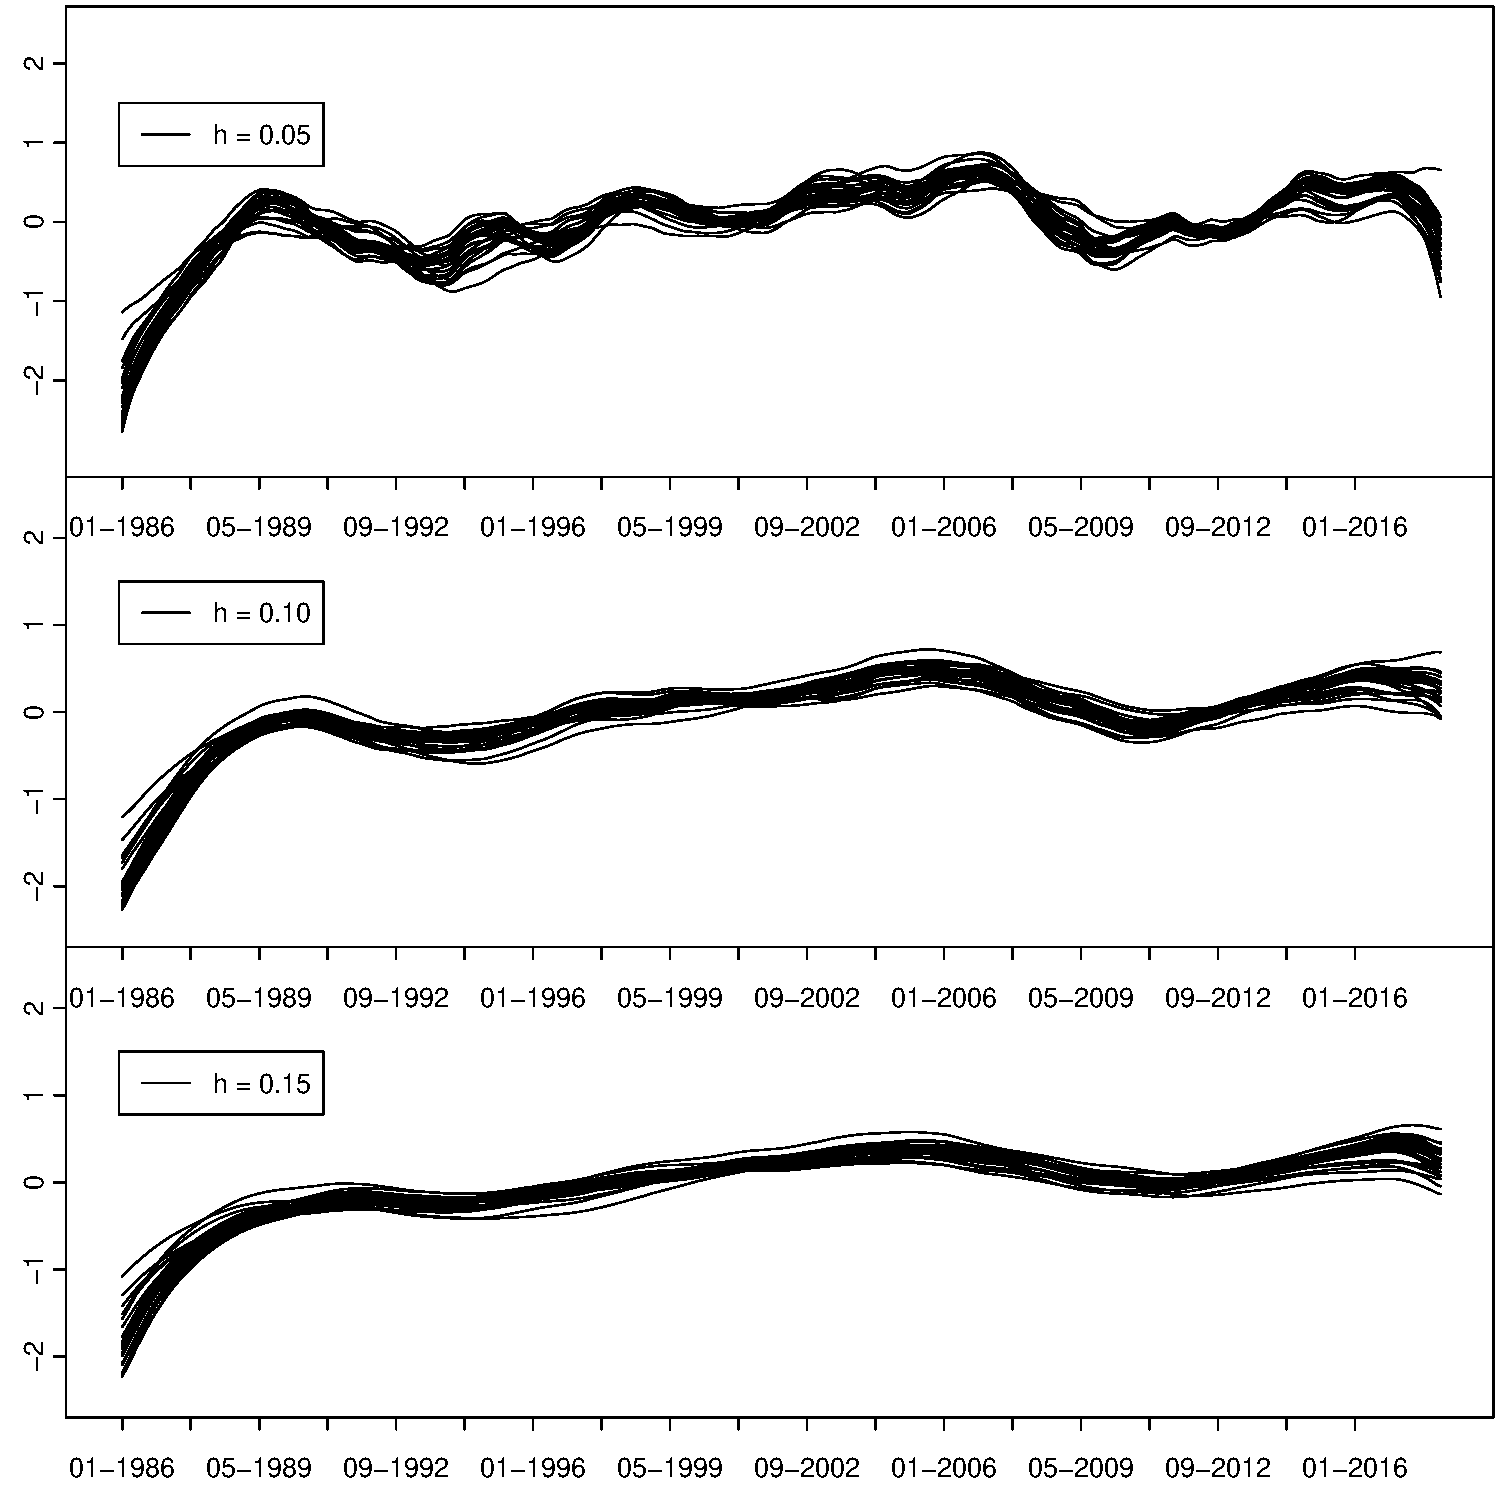
\includegraphics[width=0.8\textwidth]{Plots/stations_data.pdf}
\vspace{0.2cm}
\caption{Local linear kernel estimates of the $n=25$ time trends from the application of Section \ref{subsec-data-2}. Each panel shows the estimates for a different bandwidth $h$.}\label{plot-results-app2}
\end{figure}


To illustrate our test method from Section \ref{sec-test-equality}, we examine a dataset of monthly mean temperatures from $34$ different UK weather stations. The data are publicly available on the webpage of the UK Met Office. We use a subset of $25$ stations for which data are available over the time span from $1986$ to $2017$. We thus observe a time series $\mathcal{Y}_i = \{Y_{it}: 1 \le t \le T \}$ of length $T = 386$ for each station $i \in \{1,\ldots,25\}$. The time series $\mathcal{Y}_i$ is assumed to follow the model 
\begin{equation}\label{model2-app}
Y_{it} = \alpha_i(t) + m_i\Big(\frac{t}{T}\Big) + \varepsilon_{it}, 
\end{equation}
where $m_i$ is an unknown nonparametric time trend and $\alpha_i(t)$ is a month-specific intercept which captures the seasonality pattern in the data. We suppose that $\alpha_i(t) = \alpha_i(t + 12 \ell)$ for any integer $\ell$, that is, we have a different intercept $\alpha_i(k)$ for each month $k = 1,\ldots,12$. The test method and the underlying theory from Section \ref{sec-test-equality} can be easily adapted to model \eqref{model2-app}, which is a slight extension of model \eqref{model2}. The details are provided below. As in Section \ref{subsec-data-1}, the error process $\mathcal{E}_i = \{ \varepsilon_{it}: 1 \le t \le T \}$ is assumed to have the AR(1) structure $\varepsilon_{it} = a_i \varepsilon_{i,t-1} + \eta_{it}$ for each $i$, where $\eta_{it}$ are i.i.d.\ innovations with mean zero.  




\newpage
\bibliographystyle{ims}
{\small
\setlength{\bibsep}{0.55em}
\bibliography{bibliography}}



\end{document}
